% Created 2018-08-02 Do 20:01
\documentclass{scrartcl}

%\usepackage[latin1]{inputenc}
\usepackage[utf8]{inputenc}
\usepackage[T1]{fontenc}
\usepackage{fixltx2e}
\usepackage{graphicx}
\usepackage{longtable}
\usepackage{float}
\usepackage{wrapfig}
\usepackage{rotating}
\usepackage[normalem]{ulem}
\usepackage{amsmath}
\usepackage{textcomp}
\usepackage{marvosym}
\usepackage{wasysym}
\usepackage{amssymb}
\usepackage{hyperref}
\tolerance=1000
\author{Simon Pfaff}
\date{\today}
\title{Master\_thesis\_GER}
\hypersetup{
  pdfkeywords={},
  pdfsubject={},
  pdfcreator={Emacs 24.5.1 (Org mode 8.2.6)}}
\begin{document}

\begin{center}
\thispagestyle{empty}
\textbf{\huge Seperating the good from the bad... Exploring the genomic landscape of chloroplasts from genomic sequencing datatreduction Master Thesis}\\[1cm]
\textbf{\LARGE }\\[1cm]
{\LARGE Simon Pfaff}\\[2mm]

\includegraphics[width=.7\linewidth]{./neuSIEGEL.pdf}
{\large Julius-Maximilians-Universität Würzburg}\\[3mm]
{\large Fakultät für Biologie}
\end{center}
\cleardoublepage
\
\thispagestyle{empty}
\maketitle
\begin{center}

\includegraphics[width=.5\linewidth]{./neuSIEGEL.pdf}\\[1cm]
{\large Julius-Maximilians-Universität Würzburg}\\
{\large Betreuer: Dr. Markus Ankenbrandt}\\
{\large Betreuer: Prof. Dr. Jörg Schulz}\\
{\large Betreuer: Dr. Frank Förster}\\
{\large Lehrstuhl für Bioinformatik}\\
{\large Center for Computational and Theoretical Biology}
\setcounter{page}{1}
\clearpage
\end{center}
\tableofcontents
\clearpage
\section{Intro}
\label{sec-1}
Seperating the good from the bad\ldots{}
Exploring the genomic landscape of chloroplasts from genomic sequencing datatreduction
\subsection{Chloroplasten}
\label{sec-1-1}
Chloroplasten sind extrem wichtig, alle Pflanzen besitzen diese und nutzen sie um Energie in Form von ATP durch Photosynthese zu erzeugen.
Ihr Genom gilt als hoch konserviert, sowohl in der Gen Orientierung als auch dem Gen Inhalt \footnote{(Raubeson and Jansen 2005)}. Chloroplasten zeigen
eine auffällige Genom Struktur, das Genom ist ein einem Plasmid welches sich in drei Teile aufteilt. Dem Large Single Copy, dem 
Small Singles Copy, welche beide durch zwei Inverted repeats unterbrochen sind (Fig. 1). Chloroplasten zeigen eine viel geringere Substitutions raten
als in Genomischer DNA, diese ist noch einmal signifikant geringer in den Inverted repeat Regionen \footnote{Wolfe et al. 1987}. Dennoch zeigen sich
Einzelnucleotid-Polymorphismen (SNPs). Zudem gibt es ein seltenen Fällen eine Genwanderung von Genen auf dem IR zum SSC, wodurch ein IR weg
fallen kann, sodass solche Chloroplasten nur noch ein IR besitzen \footnote{Jansen RK, Wojciechowski MF, Sanniyasi E, Lee S-B, Daniell H. Complete plastid genome sequence of the chickpea (Cicer arietinum) and the phylogenetic distribution of rps12 and clpP intron losses among legumes (Leguminosae). Molecular phylogenetics and evolution. 2008;48(3):1204-1217. \url{10.1016/j.ympev.2008.06.013}.} . Vor allem in gezüchteten Nutzpflanzen finden sich auch 
Invertierungen des IR \footnote{Palmer et al. 1988}. Durch ihre hohe Konservierung sind Chloroplasten und ihre Gene sehr gut für Barcoding geeignet. Mit diesem
Barcoding können Pflanzen und ihre Varianten identifiziert werden. Neue Studien zeigen, dass der komplette Chloroplast selbst als ein Art "Ultra-barcode"
verwendet werden könnte, da die Variation in Chloroplasten in einer Spezies doch mehr variiert als angenommen \footnote{Kane et al. (2012)}. 
\begin{figure}
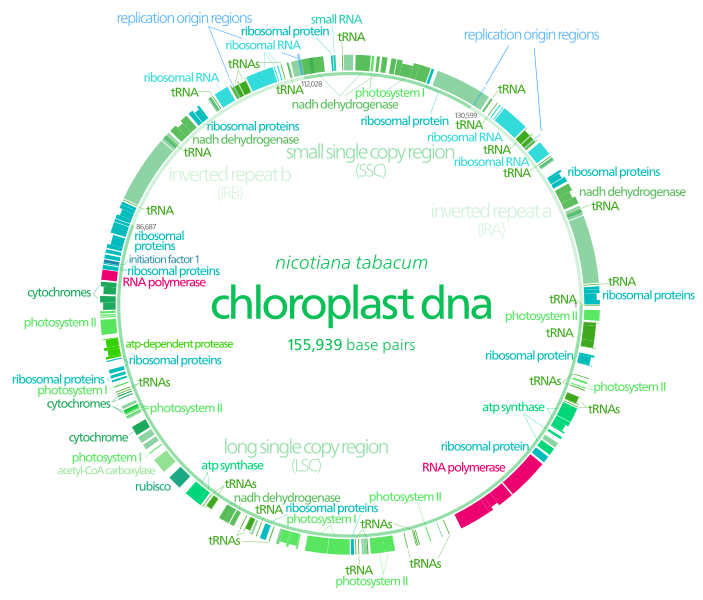
\includegraphics[width=.9\linewidth]{./703px-CtDNA.png}
\caption[Aufbau Chloroplast Genom]{\textbf{Aufbau Chloroplast Genom} Das Chloroplast Genom der Tabakpflanze, die innere Beschrifftung zeigt den B-Strang, die Äußere den A-Strang der DNA. Die Kerben visualisieren Introns}
\end{figure}
Die Gene auf einem Chloroplasten lassen sich in verschiedene Klassen einteilen. Zunächst gibt es die Gene welche für die Photosynthese wichtig sind,
hier unterteilt man nochmal in Photosystem I (psaA, psaB, etc.), Photosystem II (psbA, psbB, etc.), Cytochrome b6f (petA, petB,etc.), 
ATP Synthese (atpA, atpB, etc.), RuBisCo(rbcL) und NAD(P)H dehydrogenase Gene(ndhA, ndhB, etc.)\footnote{Vydianathan, Ravi \& P. Khurana, J \& K. Tyagi, A \& Khurana, Paramjit. (2007). An update on chloroplast genome. Plant Systematics and Evolution. 271. 101-122. 10.1007/s00606-007-0608-0.}. Die zweite Klasse beinhaltet Gene welche für den
Genetischen Apparat, also Transkription, Translation und Replikation nötig sind, sowie RNA Gene. Hierzu zählen Transfer RNA (trnH,trnK, etc.), ribosomale RNA (rrn16, rrn5, etc.), 
RNA Polymerasen (rpoA, rpoB, etc.) und ribosomale Gene (rps2, rps3, rpl2, rpl16,etc.). Die dritte und letzte Kategorie beschreibt Gene welche konservierten Open Reading Frames (ORFs)
genannt ycfs (Hypotheticalchloroplast open reading frames) und potentiell Codierende Gene wie matK und cemA\footnotemark[6]{}. Vor allem stark konservierte Gene wie rbcL und matK und cemA werden 
häufig für Barcoding oder zum berechnen von phylogenetischen Bäume verwendet.
\subsection{Big Data}
\label{sec-1-2}
Die Big Data Ära zeichnet sich vor allem durch die Flut an Daten aus welche kaum zu Bewältigen ist. Im biologischen Sinne zeichnet sich diese 
Flut an Daten vor allem durch genomische Daten aus. Durch sogenannte Hochdurchsatz Methoden in modernen Sequenzierungs Technologien wie PacBio\footnote{\url{https://www.pacb.com/}} oder Illumina\footnote{\url{https://www.illumina.com/}}
sie verwenden können sehr viele genomische Daten in kurzer Zeit für vergleichsweise wenig Geld erzeugt werden. Um dieser Daten Herr zu werden sind vor allem
Programme die diese Daten auswerten wichtig. Die Anforderung an diese Programme sind unter anderem eine hohe Geschwindigkeit und vor allem eine hohe 
Automatisierbarkeit. Um solche Programme zu entwickeln sind vor allem Kenntnisse in Informatik und in Biologie notwendig. Informatik ist wichtig um eine sinnvolle Programm Struktur 
zu entwickeln sowie natürlich das Programmieren an sich, und alles was dazugehört von Bugs fixen bis zur Optimierung der Software. Biologie ist wichtig um die oftmals komplizierten
Biologischen Fragestellungen und Sachverhalte zu verstehen.  
\subsection{Open Science}
\label{sec-1-3}
Mit der Flut der ansteigenden Daten wächst in den letzten Jahren auch immer mehr die Akzeptanz zur "Open Science".
"Open Science" bezeichnet eine Bewegung welche fordert dass Wissenschaft und alles was dazugehört, Daten, Programme, Ergebnisse öffentlich und für jedermann 
zugänglich sein soll. Befürworter dieser Bewegung argumentieren damit, dass Wissen für jedermann zugänglich sein sollte, und nicht nur für Ausgewählte oder gar
gegen Bezahlung. So steigere sich unter anderem die Akzeptanz der Wissenschaft als auch deren Glaubwürdigkeit. Da die Ergebnisse von jedem nachvollziehbar 
veröffentlicht werden müssen mit allen Rohdaten und Vorgehensweisen. Dies sei der eigentliche Gedanke hinter der Wissenschaft, sie solle jedem zugänglich sein!
Diese Bewegung findet vor allem bei jung Wissenschaftler aber auch bei älteren immer mehr Anklang. Mittlerweile gibt es mehrere Lizenz Modelle die unter
Open Science laufen. Diese Regeln wie die Daten verwendet werden dürfen oder müssen. Dies reicht von Freigeben der Daten und jeglichem Verwendungszweck bis hin
zum Zwang, dass alles was mit diesen Daten oder auch Programmen veröffentlicht wird wieder unter der gleichen Open Science Lizenz zu publizieren ist.
Alle hier verwendeten Programme und Daten sind unter Open Science Lizenzen veröffentlicht, sonnst wäre diese Arbeit garnicht möglich. 
Deswegen werden alle Ergebnisse wiederum öffentlich verwendbar sein. Denn so sollte Wissenschaft sein!  

\subsection{Daten in Daten}
\label{sec-1-4}
Bei den heutzutage geringen Kosten Daten, vor allem genomische Daten, zu erzeugen ist es nicht verwunderlich dass immer neue Daten generiert werden.
Dennoch steckt in bereits erhobenen Daten meist mehr Information als zunächst verwendet. In genomischen Daten zum Beispiel, hier findet sich meistens Daten 
von Organellen, wie Mitochondrien oder Chloroplasten, welche ihre eigene DNA besitzen. Diese sind dort zu finden da vor einer Sequenzierung häufig keine 
Kern Extraktion durchgeführt wird, da diese mehr Zeit und Geld kosten würde. Diese Organellen DNA können mit bestimmten Programmen gefiltert werden, hierfür 
wurde unter anderem der chloroExtractor programmiert. Dieser kann in genomischen Pflanzen Daten Chloroplasten DNA finden und diese verwenden um einen vollständigen
Chloroplasten bauen. Hiermit müssen somit keine neuen Sequenzierungen für Chloroplasten mehr durchgeführt werden, wenn man an Chloroplasten forschen möchte.
\subsection{Verwendete Programme und ihre Ansätze}
\label{sec-1-5}
Es gibt verschiedene Ansätze um Chloroplasten Genome bzw. ihre DNA aus genomischen Pflanzen Daten zu extrahieren. Die wohl einfachste Möglichkeit ist ein Referenz basiertes
Mapping der Daten auf einen Referenz Chloroplasten. Hierzu muss lediglich ein nah verwandter Chloroplast als Referenz benutzt werden. So können die Reads, welche auf diese Referenz
passen genommen werden und assembliert werden, mit der gleichen Referenz. Dies funktioniert allerdings nur wenn man eine passende Referenz benutzt, diese sollte von der gleichen Spezies oder
zumindest einer Nah verwandten Spezies stammen. Ein anderer Ansatz besteht darin den Chloroplasten de novo zu assemblieren, also ohne Referenz. Um diesen Ansatz zu benutzen müssen
aber zunächst die Reads mit Chloroplasten Genom aus den Daten gezogen werden. Hier gibt es wiederum verschiedene Möglichkeiten. Eine Möglichkeit ist es die Reads gegen eine Datenbank
von Chloroplasten Genen zu blasten, hierzu muss entweder eine Datenbank von Chloroplasten Genen gestellt werden oder der Benutzer muss eine Pseudo-Referenz einen sogenannten Seed angeben.
Ein Seed, was von einigen Basenpaaren bis zu einem kompletten Chloroplasten reichen kann, kann auch eingesetzt werden um durch ein reines Mapping Reads zu finden. Bei kleinen Seeds wird dieser
häufig durch gefundene Reads erweitert und eine Liste von Seed erstellt. Auch hier muss aber sichergestellt werden, dass der Seed in den Chloroplasten Daten vorhanden ist.
Von diesen Methoden gibt es auch Abwandlungen, wie z.b. das scannen der Daten durch Kmers, hier werden die Daten in verschiedene Kmers zerteilt, durch plotten dieser Kmers können
an spezifischen Stellen überrepräsentierte Kmers gefunden werden, diese überrepräsentierten Kmer spiegeln häufig Plasteome wieder. Diese sind unter anderem Chloroplasten aber auch
Mitochondrien, sie besitzen ihre eigene DNA und kommen im Schnitt häufiger vor als DNA welche im Zellkern zu finden ist. 
Abgesehen von den Ansätzen der Programme gibt es zwei verschiedene Arten von Programmen, die einen benutzen bereits vorhandene Programme wie Assambler, Mapper oder Kmer-counter. Diese 
Bauen eine Pipeline um diese Programme, sodass diese in der richtigen Reihenfolge mit den richtigen Parametern mit nur einem Befehl gesteuert werden können. Der Vorteil ist, solche Programme
sind einfacher zu warten da sie meist kleiner sind als Programme die dies nicht tun und einfacher zu Programmieren, allerdings sind sie von diesen drittanbieter Programmen abhängig und es können Probleme 
auftreten wenn diese Änderungen bzw. Updates ausgeben, weswegen meist die kompatiblen Versionen angegeben werden. Ein weiterer Nachteil, der Benutzer muss häufig weitere Programme, sogenannte Abhängigkeiten installieren
bevor er das eigentliche Programm nutzen kann. Die andere Möglichkeit ist es die komplette Maschinerie selbst zu Programmieren, dies ist sehr aufwendig und bedeutet viel Wartungsarbeit. Vorteil hier
ist das keine anderen Abhängigkeiten benötigt werden außer ein System welches das Programm verwenden kann. In dieser Arbeit wurden verschiedene Typen von Programmen verwendet.
Es wurden von allen Programmen die jeweils neusten Versionen benutzt, und wenn es zu großen Änderungen wie Bug-fixes kam auf die neuere Version gewechselt, um das bestmögliche Ergebnis für die Daten
zu erhalten.
\subsubsection{chloroExtractor}
\label{sec-1-5-1}
Der chloroExtractor (Versionen: 1.0.2, 1.0.3, 1.0.4 ) \footnote{Ankenbrand et al., (2018). chloroExtractor: extraction and assembly of the chloroplast genome from whole genome shotgun data. Journal of Open Source Software, 3(21), 464, \url{https://doi.org/10.21105/joss.00464}}\textsuperscript{,}\,\footnote{\url{https://github.com/chloroExtractorTeam/chloroExtractor}} ist ein Programm welches durch eine Kombination aus Kmer Analyse und Mapping auf bekannte Chloroplasten, Reads von Chloroplasten aus Pflanzen Sequenzierungs Daten
zu extrahieren. Es wurde 2018 vom chloroExtractorTeam veröffentlicht \footnotemark[9]{} und besteht hauptsächlich aus Perl und R Code. Es verwendet ein Pipeline Programm (PipeWrap.pm) um den richtigen Ablauf zu steuern.
Dieses Pipeline Tool wird durch eine Konfigurations Datei gesteuert, sodass ein Benutzer einfach neue Schritte einfügen könnte. Auch können hiermit einfach über ein File Parameter gesteuert werden welche dann in 
allen verwendeten Programmen gleich sind, oder einzelnen Programmen speziellen Input mitgegeben werden kann. Auch verfügt der chloroExtractor dank PipeWrap über ein Checkpoint System. Bricht der Ablauf des Programmes
ab, kann er am genau diesem Punkt wieder gestartet werden ohne das Programm von neu starten zu müssen. Zunächst verwendet der chloroExtractor Jellyfish \footnote{Guillaume Marcais and Carl Kingsford, A fast, lock-free approach for efficient parallel counting of occurrences of k-mers. Bioinformatics (2011) 27(6): 764-770 (first published online January 7, 2011) \url{10.1093/bioinformatics/btr011}} um aus den Rohdaten Kmere zu bauen, diese werden über ein R
Skript skaliert und gleichzeitig auf Chloroplasten mit Bowtie2 \footnote{Langmead B, Salzberg S. Fast gapped-read alignment with Bowtie 2. Nature Methods. 2012, 9:357-359.} gemappt. Die reads welche gemapt haben und die richtigen Kmere werden mit SPAdes\footnote{Bankevich A., Nurk S., Antipov D., Gurevich A., Dvorkin M., Kulikov A. S., Lesin V., Nikolenko S., Pham S., Prjibelski A., Pyshkin A., Sirotkin A., Vyahhi N., Tesler G., Alekseyev M. A., Pevzner P. A. SPAdes: A New Genome Assembly Algorithm and Its Applications to Single-Cell Sequencing.        Journal of Computational Biology, 2012} anschließend assembliert, SPAdes arbeitet de novo und benötigt
keine Referenz. SPAdes verwendet eine De Brujin-Graphen Methode um die reads richtig zusammen zu fügen, diese werden dann durch ein Perl Skript (fcg.pl) zu einem zirkulären Chloroplasten zusammengebaut. Dieses Skript überprüft
gleichzeitig mit BLAST+\footnote{Christiam Camacho, George Coulouris, Vahram Avagyan, Ning Ma, Jason Papadopoulos, Kevin Bealer and Thomas L MaddenEmail author, BMC Bioinformatics200910:421 \url{https://doi.org/10.1186/1471-2105-10-42}} ob es sich bei den ausgegebenen Reads wirklich um Chloroplasten handelt. Es wurden drei Verschiedene Versionen des chloroExtractors verwendet, dies brachten unter anderem Bug fixes welche das 
Programm zum Absturz brachten. Aber auch Verbesserungen am fcg.pl Skript.

\begin{figure}
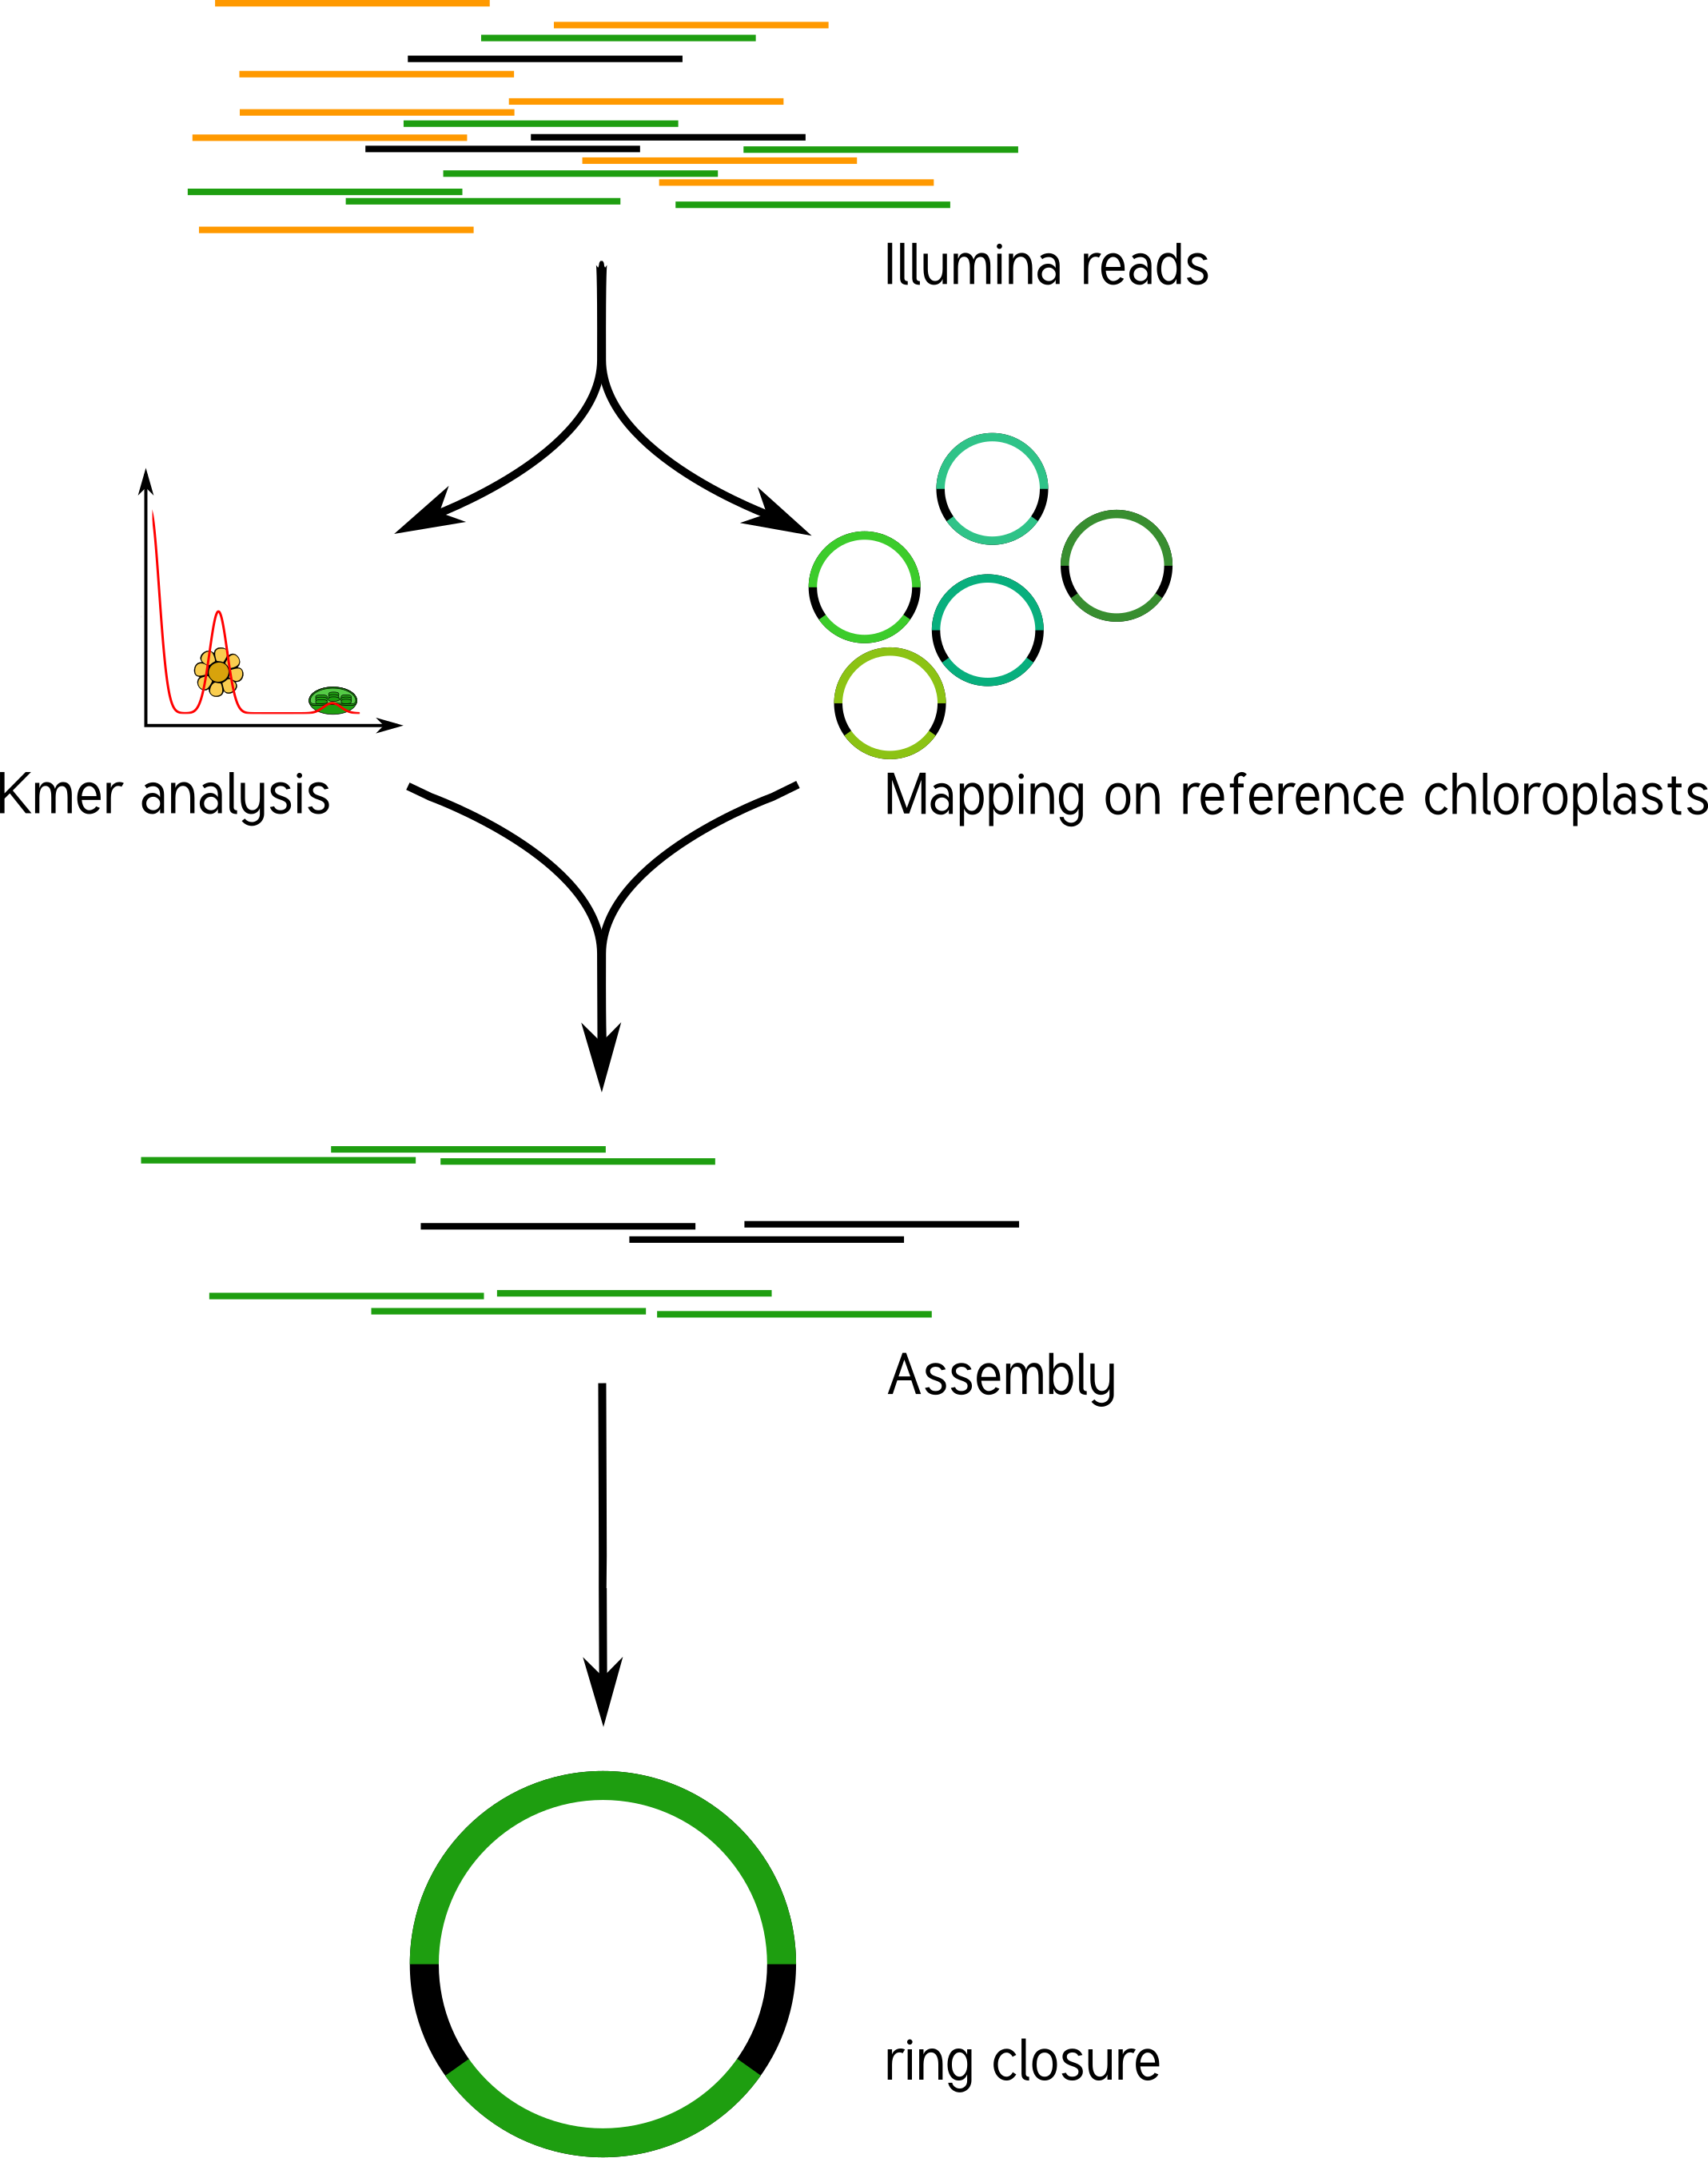
\includegraphics[width=.9\linewidth]{./workflow.png}
\caption[Ablauf des chloroExtractors]{\textbf{Ablauf des chloroExtractors} Eine kombination aus kmer Analyse und mapping auf bekannte Chloroplasten rekrutieren Chloroplasten reads um diese anschließend zu Assemblieren um anschließend einen Ringschluss herbeizuführen}
\end{figure}

\subsubsection{fast-plast}
\label{sec-1-5-2}
Fast-plast  (Version: 1.2.8) \footnote{\url{https://github.com/mrmckain/Fast-Plast}} ist ein weiteres Programm, welches verwendet wird um Chloroplasten DNA zu finden. Es ist in Perl und in C++ programmiert und verwendet auch SPAdes, 
aber zusätzlich Bowtie1 sowie Bowtie2. Auch hier wird Blast+ verwendet um die richtigen reads zu finden. 
\subsubsection{NOVOPlasty}
\label{sec-1-5-3}
Im Gegensatz zu den anderen verwendeten Programmen, benutzt NOVOPlasty (Versionen: 2.6.8. 2.6.9, 2.7.0 )\footnote{\url{https://github.com/ndierckx/NOVOPlasty}}\textsuperscript{,}\,\footnote{Dierckxsens N., Mardulyn P. and Smits G. (2016) NOVOPlasty: De novo assembly of organelle genomes from whole genome data. Nucleic Acids Research, doi: 10.1093/nar/gkw955} keine dritt Anbieter Programme. Es benötigt somit keine Abhängigkeiten von deren Programmen
und ist komplett in Perl programmiert. NOVOPlasty benutzt sogenannte seeds um Chloroplasten DNA zu finden, dies können einzelne Chloroplasten Gene sein, aber auch ein kompletter Chloroplast.
Die Verschiedenen Verwendeten Versionen versprachen Bug fixes sowie neue Features. 
\subsubsection{Org.ASM}
\label{sec-1-5-4}
Org.ASM ( Version: 1.0.00-alpha11) \footnote{\url{https://pythonhosted.org/ORG.asm/}} ist ein Programm hauptsächlich geschrieben in Python. Es versucht überrepräsentierte Sequenzen zu finden und diese zu assemblieren\footnote{\url{https://git.metabarcoding.org/org-asm/org-asm/wikis/home}}. 
Mit Hilfe eines Seeds versucht er diese Sequenzen zu finden. Da Chloroplasten und andere Organellen wie Mitochondrien in Zellen überrepräsentiert sind, vor allem
wenn man eine geringe Coverage über das Pflanzen Genom hat, sind diese somit detektierbar\footnote{\url{https://pythonhosted.org/ORG.asm/algorithms.html}}.
\subsubsection{GetOrganelle}
\label{sec-1-5-5}
GetOrganelle (Versionen: 1.9.82, 1.0.1, 1.0.3 )\footnote{\url{https://github.com/Kinggerm/GetOrganelle}}\textsuperscript{,}\,\footnote{Jian-Jun Jin*, Wen-Bin Yu*, Jun-Bo Yang, Yu Song, Ting-Shuang Yi, De-Zhu Li. 2018. GetOrganelle: a simple and fast pipeline for de novo assembly of a complete circular chloroplast genome using genome skimming data. bioRxiv, 256479. \url{http://doi.org/10.1101/256479}} verwendet zum lokieren der Chloroplasten reads ähnlich wie andere Programme Bowtie2 \footnotemark[12]{} und Blast+, nur muss hier eine Referenz mitgegeben werden. Diese wird nur hierfür
verwendet, das assemblieren hingegen geschieht de novo mit SPAdes. Wie auch beim chloroExtractor wird hier der fastg-Graph verwendet um den Chloroplasten zu finden, aber dies muss in falle 
des GetOrganelle per Hand, mit Hilfe des Programms Bandage vollzogen werden. Wie bereits erwähnt nutzt der chloroExtractor ein Perl Skript welchen diesen händischen Schritt automatisiert. 
Vom GetOrganell wurden drei Versionen verwendet. Zunächst 1.9.82, diese wurde geändert zu 1.0.1 (github commit: b390260 vom 31. März 2018) und 1.0.3, hier gab es in den verschiedenen Versionen Bugfixes.
\subsubsection{IOGA}
\label{sec-1-5-6}
Der Iterative Organellar Genome Assambly, kurz IOGA (Keine Versionsnummer vergeben, github commit: c460ea9 vom 10. Sep. 2016 )\footnote{\url{https://github.com/holmrenser/IOGA}}\textsuperscript{,}\,\footnote{Bakker et al. 2015, Herbarium genomics: plastome sequence assembly from a range of herbarium specimens using an Iterative Organelle Genome Assembly pipeline, Biol. J. Linnean Soc.} verwendet BBmap \footnote{\url{https://jgi.doe.gov/data-and-tools/bbtools/}} für das filtern und trimmen der reads, um anschließend mit SOAPdenovo2 \footnote{Luo R, Liu B, Xie Y, et al. SOAPdenovo2: an empirically improved memory-efficient short-read de novo assembler. GigaScience. 2012;1:18. \url{10.1186/2047-217X-1-18}.} und SPAdes \footnotemark[13]{} die reads zu assemblieren. 
Auch dieses Programm benötigt eine Referenz. Der IOGA ist in Python geschrieben.

\subsection{Interesse an Chloroplasten, was tun damit mit diesen Daten?}
\label{sec-1-6}
Mit der steigenden Anzahl an frei erhältlichen Chloroplasten Genomen, welche gegen ende 2016 erstmals die 1000 Genome überschritten hat\footnote{Tonti-Filippini, J. , Nevill, P. G., Dixon, K. and Small, I. (2017), What can we do with 1000 plastid genomes?. Plant J, 90: 808-818. \url{10.1111/tpj.13491}}, können immer mehr Versuche mit vielen Chloroplasten durchgeführt werden.
So ist immer noch nicht geklärt wie genau die Replikation von Plastid Genomen wie von Chloroplasten wirklich funktioniert. Wie werden Mutationen im Inverted Repeat repariert oder bei der Replikation auf beide IRs übernommen?
Da SNPs im IR immer auf beiden gefunden werden. Welche Mutationen treten am häufigsten auf und wie sind diese evtl. an die Struktur des Genoms gekoppelt \footnote{Massouh A, Schubert J, Yaneva-Roder L, et al. Spontaneous Chloroplast Mutants Mostly Occur by Replication Slippage and Show a Biased Pattern in the Plastome of Oenothera. The Plant Cell. 2016;28(4):911-929. \url{10.1105/tpc.15.00879}.}? Auch ist immer noch nicht exakt verstanden wie Chloroplasten
vererbt werden, es wird zwar angenommen das diese ähnlich wie Mitochondrien maternal vererbt werden doch gibt es bei Pflanzen auch viele Arten die biparental oder uniparental Chloroplasten vererben\footnote{Greiner S, Sobanski J, Bock R. Why are most organelle genomes transmitted maternally? Bioessays. 2015;37(1):80-94. \url{10.1002/bies.201400110}.}. Die in den letzten 
Jahren stark steigende Anzahl an Chloroplasten Genomen gibt diesen Fragestellungen neue Rohdaten die diese Probleme evtl. lösen können. Auch Probleme die nur mit kleinen Änderungen im Chloroplasten Genom zu tun haben (wie SNPs)
können so auf den Grund gegangen werden, oder auch die Adaption von verschiedenen Chloroplasten Genen in das Pflanzengenom und der daraus folgenden Änderung im Photosynthese Systems\footnote{Wicke S, Schneeweiss GM, dePamphilis CW, Müller KF, Quandt D. The evolution of the plastid chromosome in land plants: gene content, gene order, gene function. Plant Molecular Biology. 2011;76(3-5):273-297. \url{10.1007/s11103-011-9762-4}.}. Auch kann ohne große Änderung an der
kodierenden Sequenz, alleine durch Änderung an Transkriptionsfaktoren oder deren Level viel Einfluss auf solche Systeme genommen werden, welche natürlich auch mit dem Chloroplasten zusammenhängen. Wie bereits erwähnt 
eigenen sich Chloroplasten gut als Barcode Marker auch hier können Fortschritte mit mehr Daten erlangt werden. Zudem können mit vielen Chloroplasten Daten sehr gut Phylogenetische Bäume berechnet werden\footnote{Chase MW, Fay MF. Ancient flowering plants: DNA sequences and angiosperm classification. Genome Biology. 2001;2(4):reviews1012.1-reviews1012.4.}.
Dies sind alles Beispiele wie zwischen Spezien mit Hilfe von Chloroplasten Forschung betrieben werden kann. Aber auch innerhalb einer Spezies tauchen Variabilitäten auf, und dies konnte nur mit vielen verschiedenen
Chloroplasten der gleichen Spezies herausgefunden werden. So wurden beim 1001 Genom Projekt mehrere Tausend SNPs auf A.thaliana Chloroplasten gecalled\footnote{\url{http://1001genomes.org/}}\textsuperscript{,}\,\footnote{Alonso-Blanco C, Andrade J, Becker C, Bemm F, Bergelson J, Borgwardt KM, et al. 1135 genomes reveal the global pattern of polymorphism in Arabidopsis thaliana. Cell. 2016;166(2):481–491. doi: 10.1016/j.cell.2016.05.063}. 
Doch können nicht nur die Anzahl der neuen Chloroplasten Probleme lösen, schon einzelne neue Chloroplasten können sehr aufschlussreich und informativ sein. So wurde die Idee des chloroExtractors z.B. nur aus dem Grund
entworfen einen Chloroplasten aus dem Dionaea muscipula ( Venusfliegenfalle ) Genom zu extrahieren, um diesen separat zu haben um das Genom leichter zu assemblieren und annotieren. Denn es kann durchaus vorkommen
dass bei neuen Genomen, welche de novo assembliert werden müssen Verunreinigungen durch Chloroplasten auftreten können. Denn \textasciitilde{}5 - 20\% der kompletten DNA wird von Plastiden DNA ausgemacht, je nach Spezies und Gewebe\footnotemark[27]{}.


\subsection{Aufgaben in der Master Thesis}
\label{sec-1-7}
Die Aufgaben dieser Thesis ist grob in drei Teile eingeteilt. Zunächst sollen die verschiedenen Programme, der chloroExtractor \footnotemark[9]{}\textsuperscript{,}\,\footnotemark[10]{}, fast-plast\footnotemark[15]{}, IOGA\footnotemark[23]{}\textsuperscript{,}\,\footnotemark[24]{}, GetOrganelle\footnotemark[21]{}\textsuperscript{,}\,\footnotemark[22]{},
Org.ASM \footnotemark[18]{}und NOVOPlasty\footnotemark[16]{}\textsuperscript{,}\,\footnotemark[17]{} verglichen werden und herausgefunden werden welche das oder die besten Programme sind um damit so viele Chloroplasten Genome zu erzeugen wie 
möglich. Hier soll vor allem darauf geachtet werden dass die Programme Automatisierbar sind um einen hohen Durchsatz zu haben. Zudem sollen die Programme Ressourcen schonend arbeiten. 
Der zweite Teil ist das Produzieren von Chloroplasten Genomen, hierzu werden die Pflanzen Genome des 1001 Genom Projektes verwendet. Auf den so
Produzierten Chloroplasten sollen verschiedene wissenschaftliche Arbeiten durchgeführt werden, so zum Beispiel eine Varianz Analyse sowie eine Genomweite Assoziationsstudie, kurz GWAS \footnote{Korte A, Farlow A. The advantages and limitations of trait analysis with GWAS: a review. Plant Methods. 2013;9:29. \url{10.1186/1746-4811-9-29}.}.
Eine GWAS versucht bestimmte Traits, also Eigenschaften mit Genomischen Varianten zu assoziieren, um anschließend eine Aussage darüber treffen zu können ob diese Variante einen Einfluss auf diese 
Eigenschaft hat oder nicht. Hierzu werden die einzelnen Chromosomen einzeln oder als komplettes Genom angesehen, je nach Ansatz oder Fragestellung.
Auch sollte eine Struktur Varianz Analyse durchgeführt werden. Zudem könnten diese Daten benutzt werden um Chloroplasten besser als Genetische Marker zu benutzen. 
Der dritte Teil ist das Suchen nach bisher noch nicht dokumentierten Chloroplasten Genomen, hierzu sollen Daten verwendet werden welche noch keinen Eintrag in der Chloroplasten Datenbank haben.



\section{Material / Methoden}
\label{sec-2}
\subsection{Evaluation der Programme}
\label{sec-2-1}
Um die oben genannten Programme zu vergleichen habe ich mir verschiedene Ansätze überlegt.
Um zunächst zu testen wie genau die Programme funktionieren und ob diese überhaupt funktionieren,
habe ich sie auf dem Testset SRR5216995 (Arabidopsis thaliana: Col-0) mit eine Millionen reads getestet, 
dieser ist frei zugänglich bei NCBI und dient als Testset beim chloroExtractor\footnotemark[9]{}. Um eine 
Automatisierung zu erhalten muss für jedes Programm ein Dockercontainer gebaut werden, falls nicht 
schon einer vorhanden ist, letzteres trifft nur für den chloroExtractor zu. Um das Ziel zu erreichen
so viele Chloroplasten wie möglich zu extrahieren, musste eine Automatisierungslösung für alle Programme
erstellt werden, damit keine evtl. Manuelle Schritte oder Auswertungen der zeitbestimmende Schritt sind.
Um dies zu erreichen musste ich zusätzlich einige Bash Skripte (s. Anhang) schrieben welche eine volle
Automatisierung ermöglichen.   

\subsubsection{Testdaten}
\label{sec-2-1-1}
Es wurden verschiedene Größe von Dateien verwendet. So sind dies alles Illumina short read Daten, doch unterscheiden sich diese in Readlänge, Insertsize und Anzahl der Reads.

\paragraph{Simulierte Daten}
\label{sec-2-1-1-1}
Um zu Testen wie gut die verschiedenen Programme mit unterschiedlichen Anteilen von Chloroplasten DNA in
Genom Daten zurechtkommen wurden drei verschiedene Testdatensätze simuliert(Genom : Chloroplast - 1:10, 1:100, 1:1000). 
Mit diesen sollte auch getestet werden ob die Programme mit viel oder wenig Chloroplasten DNA Anteil zurecht kommen oder einen dieser Fälle 
bevorzugen. Diese Testdatensätze wurden mit ART\footnote{Weichun Huang, Leping Li, Jason R. Myers, Gabor T. Marth; ART: a next-generation sequencing read simulator, Bioinformatics, Volume 28, Issue 4, 15 February 2012, Pages 593–594, \url{https://doi.org/10.1093/bioinformatics/btr708}}\textsuperscript{,}\,\footnote{\url{https://www.niehs.nih.gov/research/resources/software/biostatistics/art/index.cfm}} erzeugt. ART wird dazu verwendet Short-reads zu erzeugen. 
Hierzu wurden Arabidopsis Thaliana (TARIR10 \footnote{\url{https://www.ncbi.nlm.nih.gov/assembly/GCF_000001735.3/}}) Daten verwendet. Mitochondrien DNA wurde nicht mit simuliert, da diese zu 
Problemen führen könnte wenn diese aufgrund ihrer ähnlichen Häufigkeit für Chloroplasten DNA identifiziert werden. 
Um die verschiedenen Verhältnisse von Genom und Chloroplasten zu bekommen wurden die Chloroplasten Daten einfach
vervielfältigt und anschließend zusammen kopiert. Hiernach wurden sie mit folgenden ART Kommandos zu short-reads simuliert.
Für die Tests wurden eine Millionen Reads pro Datei benutzt, da diese genug Chloroplasten DNA enthalten sollten.

'art\_illumina [options] -i <INPUT\_SEQ\_FILE> -l <READ\_LEN> -f <FOLD\_COVERAGE> -o <OUTPUT\_FILE\_PREFIX> -m <MEAN\_FRAG\_LEN> -s <STD\_DE>'
'1:10 : ./art\_illumina -p -i sequence-arabidopsis-thaliana-kern-chl-1zu10.fa -l 150 -f 100 -o a\_thaliana\_1\_10\_sim -m 500 -s 150'
'1:100 :  ./art\_illumina -p -i sequence-arabidopsis-thaliana-kern-chl-1zu100.fa -l 150 -f 100 -o a\_thaliana\_1\_100\_sim -m 500 -s 150'
'1:1000 :  ./art\_illumina -p -i sequence-arabidopsis-thaliana-kern-chl-1zu1000.fa -l 150 -f 100 -o a\_thaliana\_1\_1000\_sim -m 500 -s 150'

\paragraph{1001 Genom Projekt}
\label{sec-2-1-1-2}
Um einen ersten Eindruck über die Programme und deren Erfolgsrate zu bekommen wurden parallel zu den Tests mit simulierten Daten, die ersten Tests mit realen Datensätzen vorgenommen. 
Hierzu wurden Daten aus dem 1001 Genom Projekt\footnotemark[32]{} verwendet, dies sind alles Arabidopsis thaliana. Es wurden 11 Datensätze ( SRR1945435 - SRR1945445 ) verwendet. Diese sind alle
frei verfügbar und wurden von NCBI heruntergeladen. Es wurden jeweils zwei Millionen Reads pro Datei gezogen, mit 150 basen Parren pro Read.

\paragraph{GetOrganelle-Paper preprint}
\label{sec-2-1-1-3}
Um zu weitere Testdaten zu ermitteln und ein Urteil darüber zu fällen welche Programme weiter verwendet werden,
wurden 57 Datensätze welche im GetOrganelle Paper \footnotemark[22]{} verwendet wurden
auf allen Programmen getestet. In dieser Arbeit wurden bei 47 Datensätzen von 57, mit
dem GetOrganelle erfolgreich zirkuläre Chloroplasten extrahiert. Diese Daten sind auch frei zugänglich und wurden
von NCBI heruntergeladen. Gerade hier gab es einige Abweichungen in Dateigrößen. Reads reichten von 75 basen Parren 
bis zu 300 basen Parre pro Read. Es wurden hier drei Millionen Reads pro Datei verwendet, da diese im GetOrganelle Paper
auch verwendet wurden.


\subsubsection{Welche Programme werden weiter verwendet.}
\label{sec-2-1-2}
Um alle Daten aus dem 1001 Genom Projekt (1135 Datensätze) zu berechnen, mussten aufgrund 
von Hardwaretechnischen Limitierungen die besten Programme ausgewählt werden. Diese Programme müssen in
in Geschwindigkeit sowie in Erfolgs- und Fehlerrate überzeugen. Desweiteren müssen diese Programme gut automatisierbar sein, 
d.h. am besten mit nur Befehl gestartet werden können, sodass kein weiterer Aufwand anfällt. Dies gilt
vor allem auch bei der Wahl der Parameter mit denen das Programm gestartet wird. Diese können nicht 
für jeden Datensatz angepasst werden, was bedeutet dass die Standardparameter verwendet werden.
Dies ist notwendig um einen hohen Durchsatz an Berechnungen zu ermöglichen.
\paragraph{Installation \& Automatisierung}
\label{sec-2-1-2-1}
Alle Programme konnten mit Hilfe von einigen Skripts und dem erstellen eines Dockercontainers, so 
automatisiert werden das sie einen hohen Durchsatz erreichen können. Das Einzige Programm welches
einen Händischen Schritt benötigt ist der GetOrganelle, hier muss die fastg Datei in Bandage
geöffnet werden und der zirkuläre Chloroplast selbst heraus gesucht werden.
Bei den verschiedenen Skripts handelt es sich vor allem um Start-Skripts. Aber es mussten auch ein paar 
kleine Skripts verwendet werden um kleine Bugs zu fixen. So kann der IOGA keine unter Ordner verwenden da er sonnst
versucht auf Falsche Dateien zuzugreifen und abstürzt. Dies scheint ein Bug in einem Splitt Befehl zu sein. Beim GetOrganelle mussten
zusätzliche Befehle eingebaut werden damit SPAdes keine Fehlermeldungen bringt und abbricht, da er bestimmte Funktionen (hammer.py) nicht ausführen konnte
welche für eine Fehler Korrektur verwendet werden, welche GetOrganelle gar nicht nutzt. Org.ASM konnte nur erfolgreich in einem Dockercontainer
installiert werden, da dieses Programm sonnst verschiedenste Fehlermeldungen brachte. Alle Programme welche PERL verwenden, also
chloroExtractor, fast-plast und NOVOPlasty, brachten Fehlermeldungen, da innerhalb des Dockercontainers Globale Variablen nicht vollständig gesetzt waren. 
Diese Fehler waren aber nicht fatal, und konnten mit dem setzten dieser Variable leicht entfernt werden. 
Für jedes Programm wurde ein Skript geschrieben welches die Laufzeit überprüft und wenn dieses fertig ist danach eine Auswertung startet.

\paragraph{Erfolgsrate}
\label{sec-2-1-2-2}
Um zunächst zu überprüfen ob ein wirklich ein kompletter Chloroplast zusammengebaut wurden bei den ersten Testdatensätzen ein Referenz Mapping auf
TAIR10 benutzt. Hierzu wurde mit Bowtie2, später mit minimap2 der Chloroplast auf das TAIR10 chloroplasten Genom gemapt. Auch wurde mit AliTV \footnote{Ankenbrand MJ, Hohlfeld S, Hackl T, Förster F. (2017) AliTV—interactive visualization of whole genome comparisons. PeerJ Computer Science 3:e116 \url{https://doi.org/10.7717/peerj-cs.116}} 
eine Visualisierung des Mappings erstellt. Nachdem klar war das es sich bei allen ausgegeben Daten um Chloroplasten handelt, und weil diese Art der 
Auswertung schlecht Automatisierbar war wurde ein bash Skript geschrieben welche die Auswertung übernimmt. Dieses Skript überprüft die Größe des
Chloroplasten und in wie vielen Contigs der Chloroplast ausgegeben wurde. Hierzu wurde das SeqFilter\footnote{\url{https://github.com/BioInf-Wuerzburg/SeqFilter}} Skript verwendet, und anschließend über bash
Skript eine Entscheidung getroffen ob es sich um einen kompletten Chloroplasten Handelt oder nicht (s. Anhang: ev\_stat.sh). Hierzu wurden Verschiedene
Kategorien eingeführt(s. Tab. 1). Diese Auswertung wurde für dann für alle Testdaten sowie die GetOrganelle PrePrint Daten verwendet.
\begin{table}[!h]
\caption[Erfolgsraten Einteilung]{\textbf{Erfolgsraten Einteilung} Das Skript ev\_stat.sh scannt die Output Dateien und teilt diese je nach Größe und Anzahl der Contigs in verschiedene Kategorien ein. }
\begin{center}
\begin{tabular}{lrl}
Kategorie & Contigs & Basenpaare\\
\hline
Success & 1 & 110 kbp  180 kbp\\
Partial & 1 & 110 kbp  180 kbp\\
Incomp:high & 1 & 180 kbp\\
Incom:low & 1 & 110 kbp\\
 &  & \\
\end{tabular}
\end{center}
\end{table}

\paragraph{Geschwindigkeit}
\label{sec-2-1-2-3}
Einer der weniger entscheidenden aber dennoch wichtigen Punkte nach dem gefiltert wurde ist die Geschwindigkeit, 
oder besser die Laufzeit der Programme. Zunächst wurde hier die Durchschnitts zeit genommen die der Prozess zum rechnen benötigt,
anschließend wurde mit dem time linux Kommando die CPU als auch die Realzeit gemessen. Die Geschwindigkeit von Programmen mit vielen Abhängikeiten 
brauchen im Schnitt länger, da zum benutzen der Dockercontainer Singularity\footnote{\url{https://singularity.lbl.gov/}} verwendet wurde. Dieses Benötigt Zeit um den Container zu verwenden,
zudem wird Zeit in Anspruch genommen wenn viele Daten in den Container gemountet werden müssen.
\paragraph{Benötigte Ressourcen}
\label{sec-2-1-2-4}
Ein weiterer Punkt nachdem aussortiert wurde ist der benötigte RAM verbrauch. Es wurden verschiedene Größen von Dateien verwendet
um in Erfahrung zu bringen wie sich dies auf Ressourcen und Laufzeit auswirkt. Zudem wurde zum Ausführen der Dockercontainer 
Singularity \footnotemark[40]{} verwendet, welches die benötigte Laufzeit und die benötigten Ressourcen beeinflusst.


\subsection{Erzeugen von Chloroplasten aus genomischen Daten}
\label{sec-2-2}
Um so viele Chloroplasten wie möglich aus den genomischen Daten des 1001 Genom Projekts raus zu holen, wurden der fast-plast und der chloroExtractor benutzt.
Diese wurden mit Hilfe eines Dockercontainers und einigen Skripts (s. Anhang) voll automatisiert. Sodass nur ein Befehl nötig war um die komplette 
Pipeline zu starten und auszuwerten. 

\subsection{Varianz Analyse}
\label{sec-2-3}
Um mehr über die Chloroplasten und deren Verbreitung, sowie Mutationsrate und somit Varianz zu erfahren wurden zwei verschiedene Varianzanalysen durchgeführt. 
Zunächst sollte überprüft werden welche Einflüsse die Programme und ihre Strategien den Chloroplasten zu assemblieren, speziell deren Assambler auf die Varianz der 
entstehenden Chloroplasten hat. Hierzu wurden die assamblierten Chloroplasten, welche beide verwendeten Programme gemeinsam hatten verwendet. Diese Läufe wurden zunächst
zehn fach wiederholt, auch um einen Eindruck über die Reproduzierbarkeit der Ergebnisse zu bekommen. Diese Chloroplasten wurden anschließend mit minimap2 \footnote{Li, H. (2018). Minimap2: pairwise alignment for nucleotide sequences. Bioinformatics. \url{10.1093/bioinformatics/bty191}} auf das 
Referenzgenom ( TAIR10 chloroplast \footnote{\url{https://www.ncbi.nlm.nih.gov/nuccore/NC_000932.1}} ) gemapt. Hiernach wurde eine Varianzanalyse mit Samtools\footnote{Li H, Handsaker B, Wysoker A, Fennell T, Ruan J, Homer N, Marth G, Abecasis G, Durbin R, and 1000 Genome Project Data Processing Subgroup, The Sequence alignment/map (SAM) format and SAMtools, Bioinformatics (2009) 25(16) 2078-9 \footnotemark}\footnotetext[44]{DEFINITION NOT FOUND.} durchgeführt, hierzu wurde der Befehl
'mpileup/bcftools call' \footnote{Li H, A statistical framework for SNP calling, mutation discovery, association mapping and population genetical parameter estimation from sequencing data, Bioinformatics (2011) 27(21) 2987-93. \footnotemark}\footnotetext[46]{DEFINITION NOT FOUND.} verwendet. Dieser führt eine Varianzanalyse bzw. ein SNP calling durch. Die zweite Varianzanalyse wurde auf allen Chloroplasten welche aus dem
1001 Genom Projekt gebaut wurden erstellt. Auch diese wurden auf den Referenzchloroplasten mit minimap2 kartiert und anschließend mit samtools' 'mpileup' Funktion einem
SNP calling unterzogen. 

\subsection{GWAS}
\label{sec-2-4}
Häufig wird eine GWAS über das komplette Genom berechnet. Doch können auch einzelne Chromosomen oder Organellen bereits signifikante Varianten besitzen. 
So soll mit dieser GWAS der Einfluss von Chloroplasten Varianten auf Eigenschaften der A.Thaliana getestet werden. Hierzu wurden die SNP callings aus der Varianzanalyse verwendet.
Verschiedene Trait-Tabellen wurden von Arapheno\footnote{\url{https://arapheno.1001genomes.org/}}, einer Trait Datenbank für A.Thaliana, heruntergeladen und zusammen mit den Varianzanalyse Daten in ein R\footnote{\url{https://www.r-project.org/}} Skript gegeben.
Dieses R Skript nutzt zunächst vcfR\footnote{\url{https://cran.r-project.org/web/packages/vcfR/index.html}}, ein R Paket, um die verschiedenen VCF (Variance Calling File) Daten einzulesen. Anschließend ruft es ein weiteres R Skript auf welches
freundlicher weiße von Korte et. al\footnotemark[34]{} zur Verfügung gestellt wurde und eine GWAS Analyse durchführt.

\subsection{Struktur Varianz Analyse}
\label{sec-2-5}
Wie bereits erwähnt können Chloroplasten auch verschiedene Strukturelle Änderungen evolvieren. Diese sind durch die Rohdaten, welche meist short-reads sind, nicht aufzudecken.
Da diese zu kurz sind um komplette Struktur Varianten zu überspannen.\footnote{1001 Genomes Consortium 1,135 genomes reveal the global pattern of polymorphism in Arabidopsis thaliana. Cell. 2016;166:481–491. [PubMed]}
Hierzu könnten nun die komplett de novo Assemblierten Chloroplasten verwendet werden. 

\subsection{Neue Chloroplasten}
\label{sec-2-6}
Um neue Chloroplasten zu finden, welche noch nicht in der CP-Base \footnote{\url{http://rocaplab.ocean.washington.edu/old_website/tools/cpbase}}\textsuperscript{,}\,\footnote{\url{http://rocaplab.ocean.washington.edu/tools/cpbase_test/}} Datenbank sind, wurde eine Liste von Möglichen Daten von NCBI mit CP-Base verglichen. Nur 49 Datensätze waren ohne 
Eintrag in CP-base und hatten somit noch keinen Dokumentierten Chloroplasten. Auf diese 49 Datensätze wurden sowohl der chloroExtractor als auch der fast-plast angewendet. 
Um die NCBI liste von Interessanten Daten zu erhalten wurde mit folgendem Befehl gesucht: 
' ((((((("green plants"[orgn]) AND "wgs"[Strategy]) AND "illumina"[Platform]) AND "biomol dna"[Properties]) AND "paired"[Layout]) AND "random"[Selection])) AND "public"[Access]'
Mit einem Skript (s. Anhang, cpbase.sh) wurden alle Spezies Einträge von CP-base geladen welche einen Chloroplasten besitzen. Anschließend wurde mit einem folgendem Perl-Einzeiler
die Datensätze herausgegeben welche noch keinen Eintrag in CP-base haben.
'perl -F"," -ane 'print if \$F\footnotemark[35]{}>399 and \$F\footnotemark[3]{}>999999' SraRunInfo\_plants.csv | grep -vf species\_cpbase.list | sort -u -t, -k29,29 | shuf'


\section{Ergebnisse}
\label{sec-3}
\subsection{Automatisierung}
\label{sec-3-1}
Um eine Automatisierung aller Programme zu erreichen wurde für jedes Programm ein Dockercontainer gebaut welcher mit Singularity verwendet wird. Zudem wird die komplette Auswertung von Skripts 
übernommen. Um dies zu Bewerkstelligen wurden mehrere Skripte geschrieben welche sich gegenseitig aufrufen um den kompletten Ablauf sicherzustellen. 
Das einzige Skript welches aktiv ausgeführt werden muss ist das run\_SRRchl.sh. Dieses Skript setzt Links zu anderen Skripts, zum einen zwei Auswertungs Skripts (ev\_stat.sh und percent\_stat.sh) und
zu einem Skript namens cp\_skript.sh. Dieses cp\_skript übernimmt den kompletten Aufbau der Ordner Struktur, und linkt all die Skripts die jedes Programm braucht, so brauchen IOGA und GetOrgranelle
eine Referenz, diese wird von diesem Skript in die passenden Ordner kopiert. Auch kopiert und führt dieses cp\_skript.sh das Skript aus welches die NOVOPlasty Konfigurationsdatei automatisiert für jeden
Datensatz schreibt (make\_NP\_config.pl). Für jeden Datensatz wird so ein Ordner erzeugt mit jeweils dem Programm als Unterordner. In jedem Unterordner werden die roh Daten verlinkt, sowie für jedes Programm
das passende Evaluierungs Skript und Run Skript. Als letztes linkt es sbatch\_run\_all.sh und ev\_all.sh in den jeweiligen Datenordner. Diese werden nun vom run\_SRRchl.sh Skript ausgeführt. Das sbatch\_run\_all.sh
Skript geht nun in jeden Unterordner und startet die jeweiligen Programme über sbatch und deren run Skript. Zudem startet es auch die Dazugehörigen Evaluierungs Skripte, welche auch gleichzeitig als Überwachungs
Skript dienen. Sobald der Slurm Job fertig ist, startet das Evaluierungs Skript des jeweiligen Programmes damit, die Finale Output Datei zu überprüfen und diese in eine der vier Erfolgs Kategorien einzuteilen. Zudem
schiebt es alle Dateien welche keine Log Dateien oder Finale Output Dateien sind in einen raw\_Programm Ordner, damit dieser mit dem clear\_skript.sh gelöscht werden kann, falls diese Daten nicht mehr benötigt werden.
Sobald alle Datensätze fertig sind wird mit dem ev\_stat.sh Skript eine Datei mit einer Erfolgstabelle mit jedem Programm. Percent\_stat.sh kann dann genutzt werden um eine Zusammenfassung über alle Datensätze zu erhalten.


\textbf{TODO: DIAGRAMM ABLAUF}

\subsection{Daten: Simulierte Daten}
\label{sec-3-2}
Die Simulierten Daten, welche mit ART\footnotemark[35]{}\textsuperscript{,}\,\footnotemark[36]{} erzeugt wurden um das verhalten der Programme bei verschiedenen Verhältnissen zu testen, konnten von drei Programmen, dem chloroExtractor, fast-plast und Org.ASM 
bei allen drei Datensätzen geschafft werden. Diese bauen einen vollständigen zirkulären zu bauen. NOVOPlasty baut zwar auch einen kompletten Chloroplasten doch gibt dieser 
nur die drei verschieden contigs aus (IR, SSC, LSC), und schafft es nicht diese in einen zirkulären Chloroplasten zu vereinen. GetOrganelle wie auch der IOGA schaffen es nicht die
simulierten Datensetz zusammen zu bauen da sie mit einem Fehler abbrechen oder wie im falle des IOGA nach zwei Wochen Laufzeit abgebrochen werden. (s. Tabelle 1) 

\begin{table}[!h]
\caption[Test Datensatz: Simmulierte Daten]{\textbf{Test Datensatz: Simmulierte Daten} S steht für Success, E für Error, die angegebene Zahl steht für die anzahl der Contigs. Bis auf IOGA und GetOrganelle konnten alle anderen Programme die Simmulierten Daten zu einem Chloroplasten zusammenbauen, auch wenn im Falle des NOVOPlasty nicht zirkulär. Die IOGA Läufe mit "-" wurden nach zwei Woche Laufzeit abgebrochen.}
\begin{center}
\begin{tabular}{rllllll}
Sim(Genome:Chloroplast) & CE & FP & NP & GO & OA & IOGA\\
 &  &  &  &  &  & \\
\hline
1:10 & S & S & S-3 & E & S & E\\
1:100 & S & S & S-3 & E & S & -\\
1:1000 & S & S & S-3 & E & S & -\\
\end{tabular}
\end{center}
\end{table}

\subsection{Daten: 1001 Genom Projekt, 11 Testdatensätze}
\label{sec-3-3}
Aus den Daten des 1001 Genom Projekts \footnotemark[32]{}\textsuperscript{,}\,\footnotemark[33]{} wurden zunächst elf Testdatensätze verwendet um auch reale Daten auf allen Programmen zu Testen.
Von den elf Testdatensätzen des 1001 Genom Projekts konnten sechs verschiedene vollständige zirkuläre Chloroplasten zusammengebaut werden. Von diesen
sechs bringt der fast-plast fünf ein und der chloroExtractor einen. Keines der anderen Programme konnte einen weiteren 
zirkulären Chloroplasten erzeugen (s. Tab.3). Diese elf Datensätze wurden per Hand ausgewertet, keiner dieser elf Datensätze konnte einwandfrei mit Bandage
zu einem zirkulären Chloroplasten gebaut werden, da immer kein Ringschluss vorhanden war.

\begin{table}[!h]
\caption[Test Datensatz: 1001 Genom Project, 11 Datensätze]{\textbf{Test Datensatz: 1001 Genom Project} S steht für Success, E für Error, I für Incomplete, die angegebene Zahl steht für die Anzahl der Contigs. Sechs verschiedene Chloroplasten konnten zu einem zirkulären Chloroplasten zusammengebaut werden, dabei werden bereits fünf vom fast-plast abgedeckt und einer wird von chloroExtractor beigesteuert. Felder mit einem "-" wurden Abgebrochen da sie nach einer Woche noch nicht fertig waren.}

\begin{center}
\begin{tabular}{llllllll}
SRA & CE & FP & NP & GO & OA & IOGA & \\
 &  &  &  &  &  &  & \\
\hline
SRR1945435 & I-5 & I & I-4 & I & E & I-6 & \\
SRR1945436 & I-6 & S & I-3 & I & I & I-8 & \\
SRR1945437 & I-5 & I & I-4 & I & I & I-10 & \\
SRR1945438 & S-3 & S & I-6 & I & E & I-10 & \\
SRR1945439 & I-4 & S & I-1 & I & I & I-10 & \\
SRR1945440 & I-4 & S & E & I & E & I-9 & \\
SRR1945441 & I-5 & S & E & I & I & I-6 & \\
SRR1945442 & I-4 & I & I-1 & I & - & - & \\
SRR1945443 & S & I & I-2 & I & I & I-8 & \\
SRR1945444 & I-4 & I & E & I & I & I-8 & \\
SRR1945445 & I-4 & I & E & I & E & I\_7 & \\
\end{tabular}
\end{center}
\end{table}

\subsection{Daten: GO-Preprint}
\label{sec-3-4}
Um mehr Daten zu testen, wurden alle 57 Datensätze des GetOrganelle Papers \footnotemark[22]{} benutzt. Da der GetOrganelle diese Daten eigentlich erfolgreich schaffen sollte
wurde hier versucht mit dem fcg.pl Skript des chloroExtractors eine Automatisierung der Daten zu erwirken. Doch versucht der GetOrganelle zunächst die die fastg-Graphen
zu verbessern, dies führt dazu dass das fcg.pl Skript nicht mehr funktioniert. So wurden die fastg-Graphen aus SPAdes direkt verwendet, doch ergaben sich hier leider nur
zwei Datensätze als zirkuläre Chloroplasten. Auf Nachfrage beim GetOrganelle Team, hieß es dass wenn es notwendig war alle Parameter angepasst wurden und dass alle 
Chloroplasten per Hand aus Bandage geholt wurden. 
Von 57 Datensätzen, welche im GetOrganelle Paper verwendet wurden, konnten 40 mit allen Programmen fertig gestellt werden (s. Tab. 4).
Alleine der fast-plast hat dabei 31 Stück zu einem zirkulären Chloroplasten zusammengebaut. Zusammen mit den 14 des chloroExtractors
konnten die 40 geschafften Chloroplasten komplett abgedeckt werden.

\begin{table}[!h]
\caption[Test Datensatz: GetOrganelle Preprint, 11 Datensätze]{\textbf{Test Datensatz: GetOrganelle Preprint} 40 von 57 Datensätze konnten komplett gelöst werden. 31 Datensets konnten mit dem fast-plast zu einem Chloroplasten gebaut werden, die 14 die der chloroExtractor schafft enthalten die restlichen 9 um auf alle 40 Chloroplasten zu kommen. Somit konnten mit zwei Programmen 74\% gelöst werden.}
\begin{center}
\begin{tabular}{lrlrrrrl}
Tool & SUCCESS & \% & ERROR & PARTIAL & INCOMPl & NO\_PAIR & Total\\
CE & 14 & \textasciitilde{}26\% & 11 & 17 & 12 & 3 & \\
FP & 31 & \textasciitilde{}57\% & 0 & 18 & 5 & 3 & \\
GO & 2 & \textasciitilde{}4\% & 21 & 26 & 5 & 3 & \\
IOGA & 0 & \textasciitilde{}0\% & 22 & 28 & 4 & 3 & \\
NP & 7 & \textasciitilde{}13\% & 19 & 8 & 20 & 3 & \\
OA & 11 & \textasciitilde{}20\% & 36 & 4 & 3 & 3 & \\
Summary & 40 & \textasciitilde{}74\% & - & - & - & 3 & 57\\
\end{tabular}
\end{center}

\end{table}


\subsection{Die besten Programme: fast-plast und chloroExtractor}
\label{sec-3-5}
Da aus Zeitlichen und Hardware Technischen gründen nicht alle Programme weiterverwendet werden konnten, wurde nach Erfolgsrate, Geschwindigkeit und benötigten Ressourcen
gefiltert, am wichtigsten war aber die Automatisierbarkeit der Programme. Bis auf der GetOrganelle konnte für jedes Programm eine Automatisierbarkeit
erwirkt werden. Der GetOrganelle benötigt das öffnen der fastg Datei in einem Visualisierungs Programm für fastg-Graphen, hier wird Bandage empfohlen.
Bandage hat allerdings eine schlechte Kommandozeilen Anbindung wodurch auch keine Automatisierbarkeit durch Skripts erfolgen konnte.
Es wurde auch versucht mit dem fcg.pl Skript aus dem chloroExtractor, welches genau diesen Schritt im chloroExtractor automatisiert, zu verwenden um auch beim
GetOrganelle eine Automatisierbarkeit zu erreichen. Doch führte dies nur bei sehr wenigen Daten zum Erfolg, da der GetOrganelle die von SPAdes erstellte 
fastg Datei versucht zu verbessern, und die getrimmte Datei nicht mehr vom fcg.pl Skript verwendet werden kann. Dies passiert wohl weil der GetOrganelle beim verbesserten
fastg Graphen versucht Namen und Sequenzen anzupassen, womit das fcg.pl Skript nicht zurrecht kommt. Es wurde auch versucht die roh fastg Dateien des GetOrganelle zu benutzen
dies ergab zwar eine Automatisierbarkeit, doch würden so Teile des GetOrganelles, nämlich das verbessern der fastg Datei unterschlagen.
Die Laufzeiten der Programme unterscheiden sich sehr, von 30 Minuten bis über eine Stunde, auch die RAM werte sind sehr unterschiedlich, diese
reichen von wenigen 20 Gigabyte bis zu 60 Gigabyte. All diese Werte sind Durchschnittswerte, da verschiedene Größen von Dateien als Eingabe verwendet wurden. Da nicht alle
Dateien die gleiche Anzahl an Reads hatten, sowie die Größen der einzelnen Reads sich unterschieden. Diese reichten von 75 Basen paare bis zu 300 Basen paare, Anzahl der Reads
und somit Größe der Dateien reichten von eine Millionen Reads bis zu drei Millionen Reads. Die Laufzeiten sind, vor allem bei Programmen mit vielen Abhängigkeiten, erhört. Da zum nutzen
der Dockercontainer Singularity \footnotemark[40]{} verwendet wurde.    
\begin{table}[!h]
\caption[Laufzeit und Ressourcenverbrauch]{\textbf{Laufzeit und Ressourcenverbauch} Alle Laufzeiten sind Durchschnittswerte, RAM werte zu Peakzeiten. Die Laufzeiten reichen von 30 Minuten (chloroExtractor) bis zu 100 Minuten (IOGA), die RAM nutzung unterscheidete sich auch erheblich, diese reichen von 20 GB (chloroExtractor) bis hin zu 60 GB (fast-plast). Aufgrund der Nutzung von verschieden großen Datensätzen können nur Durchschnittswerte Angegeben werden.}
\begin{center}
\begin{tabular}{lll}
Tool & Laufzeit & RAM\\
\hline
CE & \textasciitilde{}  30 min & \textasciitilde{} 20 GB\\
FP & \textasciitilde{}  60 min & \textasciitilde{} 60 GB\\
GO & \textasciitilde{}  40 min & \textasciitilde{} 50 GB\\
IOGA & \textasciitilde{} 100 min & \textasciitilde{} 40 GB\\
NP & \textasciitilde{}  30 min & \textasciitilde{} 30 GB\\
OA & \textasciitilde{}  60 min & \textasciitilde{} 30 GB\\
 &  & \\
\end{tabular}
\end{center}
\end{table}
Die Programme welche in oben genannten Punkte überzeugt haben sind der fast-plast und der chloroExtractor. Der fast-plast benötigt zwar die 
meisten Ressourcen und ist nicht der schnellste, aber hat mit Abstand die größte Erfolgschance. Zudem ist er voll automatisierbar und erreicht 
dies mit den vorgegebenen Standard Parametern. Als zweites Programm wird der chloroExtractor verwendet, dieser ist schnell, Ressourcen arm und hat nach dem
fast-plast die zweithöchste Erfolgsrate. Mit beiden Programmen konnten alle 40 von 57 Chloroplasten der GetOrganelle-Preprint Daten berechnet werden.
Auch die anderen Daten zeigen dass es keinen Vorteil bringt ein drittes Programm mit zu verwenden, da keines der anderen Programme einen
Chloroplasten finden konnte welche nicht schon durch den fast-plast oder den chloroExtractor gefunden wurde. Zudem haben diese beiden Programme die wenigsten
Probleme bei der Handhabung wie auch bei der Installation zu beginn gemacht. Sie sind durch die gegebenen Parameter einfach zu verwenden und zu Automatisieren.
Die von den Programmen geschriebenen Log Dateien sind einfach gehalten um dem Ablauf zu folgen und klar verständlich, der fast-plast gibt sogar drei dieser
Dateien aus, da er unterscheidet zwischen Warn- und Fehlermeldungen und Standard Meldungen, und eine Datei für den Output der eingebundenen Programme. 
Der chloroExtractor gibt seine Kompletten Meldungen über ein übergeordnetes Programm aus, welche den Ablauf steuert. Dieses Programm gibt alles auf STDERROR aus und 
kann damit einfach mit geloggt werden, oder wie in diesem Fall über die slurm Datei, welche von dem verwendeten queueing System ausgegeben wird. 
Diese beiden Programme wurden auf allen Daten des 1001 Genom Projekts laufen gelassen, um möglichst viele Chloroplasten zu generieren. 
\subsection{1001 Genom Projekt}
\label{sec-3-6}
Ziel so viele Chloroplasten wie möglich vollautomatisch aus kompletten Genom Datensätze zu erzeugen, wofür zwei Programme ausgewählt worden sind, wurde zunächst auf Datensätzen 
des 1001 Genom Projekt versucht.
Von den 1135 Datensätzen welche im 1001 Genom Projekt gesammelt wurden, konnten 946 Datensätze erfolgreich von NCBI heruntergeladen werden. Die restlichen 189 konnten nicht richtig heruntergeladen werden aufgrund von Downloadfehlern. 
Zudem waren 47 Datensätze keine paired end Datensätze, und konnten deshalb nicht verwendet werden. Von diesen 899 restlichen Datensätzen konnten mit dem fast-plast und dem chloroExtractor 303 komplette zirkuläre Chloroplasten 
vollautomatisch gebaut werden, dies entspricht etwa 34\%. (Tab. 4). 
\begin{table}[!h]
\caption[Datensatz: 1001 Genom Project]{\textbf{Datensatz: 1001 Genom Project} SUCCESS, echte zirkuläre Chloroplasten. Error, Fehler oder Abbrüche im Programm. Partial, keine zirkulären Chloroplasten aber contigs richtig identifiziert. Incomplete, Nicht richtig identifizierte Chloroplasten.}
\begin{center}
\begin{tabular}{lrlrrrll}
Tool & SUCCESS & \% & ERROR & PARTIAL & INCOMPLETE & NO\_PAIR & Total\\
CE & 136 & \textasciitilde{}15\% & 54 & 3 & 706 &  & \\
FP & 266 & \textasciitilde{}30\% & 29 & 11 & 593 &  & \\
Summary & 303 & \textasciitilde{}34\% & - & - & - & 47 & 946\\
\end{tabular}
\end{center}
\end{table}

\subsection{Varianz Analyse}
\label{sec-3-7}
Um die Varianz Analyse durchzuführen und vor allem zu überprüfen ob die Assambler bzw. die Programme an sich einen Einfluss darauf haben, indem sie z.B. zufällige Seeds verwenden oder zufällige Daten bevorzugen, wurden 89 Datensätze
der 1001 Genom Projektes verwendet. Diese 89 Datensätze zeichnen sich dadurch aus, dass sowohl der chloroExtractor als auch der fast-plast diese zu vollständigen Chloroplasten zusammengebaut haben. Diese Datensätze
wurden noch zehn weitere Male berechnet. So wurden auf elf mal 89 Datensätzen überprüft welche Einflüsse die Programme auf die Varianz haben. Der chloroExtractor und somit der Assambler SPAdes brachte bei allen elf
Durchläufen die exakt gleichen Sequenzen heraus. Dieses Programm arbeitet also 100\% Reproduzierbar. Im Gegensatz dazu der fast-plast, dieser schaffte es nicht einmal bei allen elf Durchläufen alle Chloroplasten wieder
korrekt zusammen zubauen, bei bis zu neun verschiedenen Datensätzen konnte kein Erfolgreiches Ergebnis erzielt werden. Interessanter weiße waren nicht immer die selben Datensätze betroffen, so konnten bei einigen Durchläufen
ein Erfolg erreicht werden, bei dem nächsten aber nicht. Ob dies ein Zufalls Effekt des Programms oder der verwendeten Rechner-Infrastruktur ist, konnte nicht überprüft werden.
Die zweite Varianz Analyse bzw. SNP calling wurde auf allen Erfolgreich zusammengebauten Chloroplasten durchgeführt. Das SNP calling ergab das auf allen 303 Chloroplasten insgesamt 2128 SNPs gefunden wurden. 
Diese Ergebnisse werden für die GWAS Analyse verwendet.
\subsection{GWAS}
\label{sec-3-8}
Die GWAS Analyse, welche mit den 303 kompletten Chloroplasten aus den Daten des 1001 Genom Projekts und den 2128 gefunden SNPs durchgeführt wurde, konnte nur auf zwei verschieden Traits berechnet werden. Dies waren 
die Eigenschaften Flowering Time nach 16 Stunden und Flowering Time nach 18 Stunden. Dies sind die beiden Traits am besten untersucht sind und deswegen auch die meisten Daten beinhalten. Für alle anderen Traits konnten
keine Berechnungen erstellt werden da die Datenmenge nicht für eine GWAS ausreichend ist. Zudem konnte für beide berechneten Traits keine Signifikanz für einen SNP gefunden werden.
\subsection{Struktur Varianz Analyse}
\label{sec-3-9}
Für die Struktur Varianz Analyse konnten keine Ergebnisse erzielt werden, Grund hierfür war unter anderem fehlende Zeit. Aber auch konnten keine guten Programme gefunden werden welche mit kompletten Chloroplasten
umgehen konnten, die meisten nutzten direkt Illumina short reads. 

\section{Diskussion}
\label{sec-4}
\subsection{}
\label{sec-4-1}


\section{Referenzen}
\label{sec-5}

\section{Abbildungs- und Tabellenverzeichnis}
\label{sec-6}
\listoffigures

\listoftables
\section{Anhang}
\label{sec-7}
\section*{Eigenständigkeitserklärung}
ERKLÄRUNG gemäß ASPO § 21 Abs. 10\\[10mm]
Hiermit versichere ich, dass ich vorliegende Arbeit selbstständig verfasst, keine anderen als
die angegebenen Quellen und Hilfsmittel benutzt und die Arbeit bisher oder gleichzeitig
keiner anderen Prüfungsbehörde unter Erlangung eines akademischen Grades
vorgelegt habe.\\[20mm]
Würzburg, \today \hfill Simon Pfaff
\clearpage
% Emacs 24.5.1 (Org mode 8.2.6)
\end{document}
